\documentclass[12pt, twoside]{article}
\usepackage[letterpaper, margin=1in, head=30pt, headsep=0.1in]{geometry}
\usepackage[english]{babel}
\usepackage[utf8]{inputenc}
\usepackage{amsmath}
\usepackage{amsfonts}
\usepackage{amssymb}
\usepackage{tikz}
%\usetikzlibrary{quotes, angles}

\usepackage{graphicx}
\usepackage{enumitem}
\usepackage{multicol}

\newif\ifmeta
\metatrue %print standards and topics tags

\title{Regents Geometry}
\author{Chris Huson}
\date{October 2021}

\usepackage{fancyhdr}
\pagestyle{fancy}
\fancyhf{}
\renewcommand{\headrulewidth}{0pt} % disable the underline of the header
\raggedbottom


\fancyhead[LE]{\thepage}
\fancyhead[RO]{\thepage \\ Name: \hspace{4cm} \,\\}
\fancyhead[LO]{BECA / Dr. Huson / Geometry 04 Analytic Geometry}

\begin{document}

\subsubsection*{4.4 Slope}
\begin{enumerate}
\item Do Now: In the diagram below, $\overline{JK}$ has endpoints $J(-2,1)$ and $K(4,9)$.
\begin{enumerate}
  \item Find the coordinates of the midpoint $M$ of $\overline{JK}$. Mark and label it on the graph.
  \item Find the length $JK$
\end{enumerate}
  \begin{flushright}
    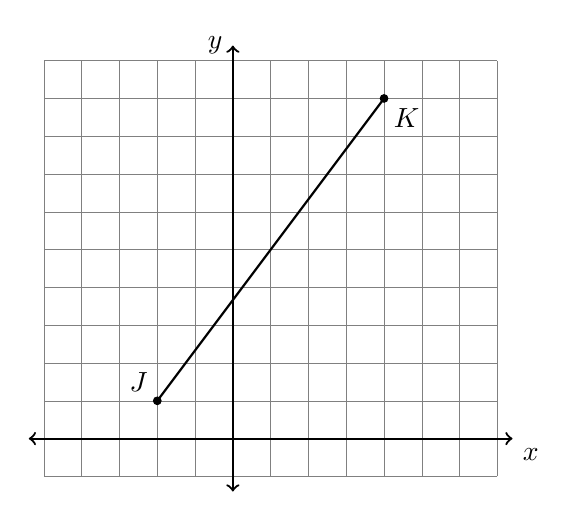
\begin{tikzpicture}[scale=.48]
      \draw [help lines] (-5,-1) grid (7,10);
      \draw [thick, <->] (-5.4,0) -- (7.4,0) node [below right] {$x$};
      \draw [thick, <->] (0,-1.4)--(0,10.4) node [left] {$y$};
      \draw [thick] (-2,1)--(4,9);
      \draw [fill] (-2,1) circle [radius=0.1] node[above left] {$J$};
      \draw [fill] (4,9) circle [radius=0.1] node[below right] {$K$};
    \end{tikzpicture}
  \end{flushright} \vspace{2cm}

\item The point $B$ is two thirds of the way from $A=-1$ to $C=5$. Find the coordinate of $B$. Mark and label $B$ on the graph of $\overleftrightarrow{AC}$. \\[1cm]
  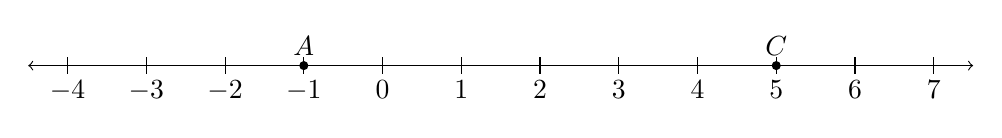
\begin{tikzpicture}
    \draw [<->] (-4.5,0)--(7.5,0);
    \foreach \x in {-4,...,7} %2 leading for diff!=1
      \draw[shift={(\x,0)},color=black] (0pt,-3pt) -- (0pt,3pt) node[below=5pt]  {$\x$};
      \draw [fill] (-1,0) circle [radius=0.05] node[above] {$A$};
      \draw [fill] (5,0) circle [radius=0.05] node[above] {$C$};
  \end{tikzpicture}
  \vspace{1cm}

  \item Point $P$ partitions $\overline{MN}$, $M=-4$ and $N=6$, in the ratio $3:2$. Find the value of point $P$. Mark and label $P$ on the graph. \\[1cm]
  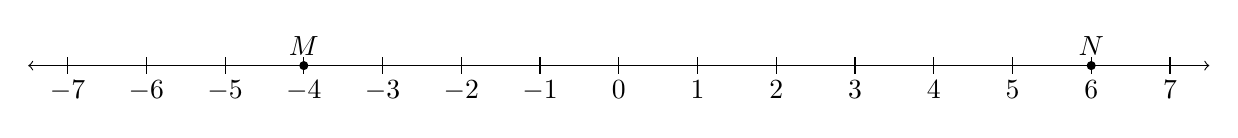
\begin{tikzpicture}
    \draw [<->] (-7.5,0)--(7.5,0);
    \foreach \x in {-7,...,7} %2 leading for diff!=1
      \draw[shift={(\x,0)},color=black] (0pt,-3pt) -- (0pt,3pt) node[below=5pt]  {$\x$};
      \draw [fill] (-4,0) circle [radius=0.05] node[above] {$M$};
      \draw [fill] (6,0) circle [radius=0.05] node[above] {$N$};
  \end{tikzpicture}

\newpage
\subsubsection*{The slope of a line}
``rise over run'': $\displaystyle m=\frac{y_2-y_1}{x_2-x_1}$

\item Find the slope of the line through the points $A(2,3)$, $B(8,5)$.
\begin{flushleft}
  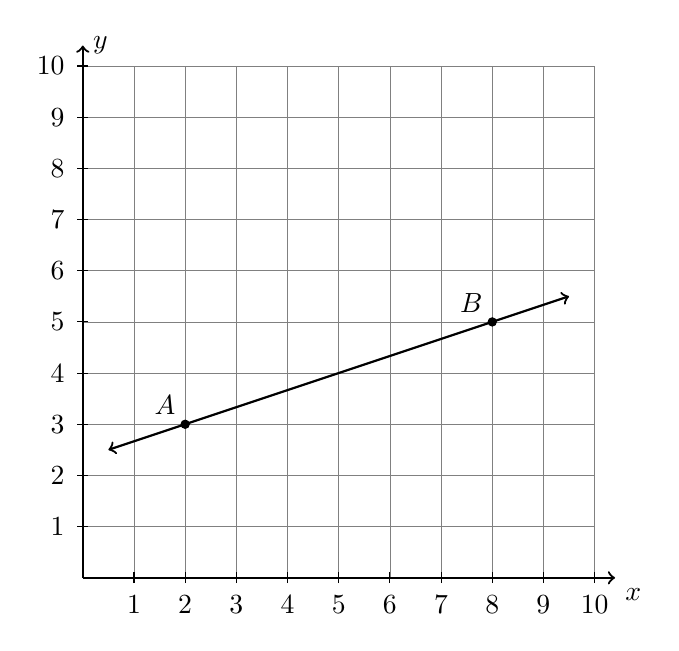
\begin{tikzpicture}[scale=.65]
    \draw [help lines] (0,0) grid (10,10);
    \draw [thick, ->] (0,0) -- (10.4,0) node [below right] {$x$};
    \draw [thick, ->] (0,0)--(0,10.4) node [right] {$y$};
    \foreach \x in {1,...,10}
    \draw[shift={(\x,0)}] (0pt,-3pt)--(0pt,3pt) node[below=5pt] {$\x$};
    \foreach \y in {1,...,10}
    \draw[shift={(0,\y)}] (-3pt,0pt)--(3pt,0pt) node[left=5pt] {$\y$};
    \draw [thick, <->] (0.5,2.5)--(9.5,5.5);
    \draw [fill] (2,3) circle [radius=0.08] node[above left] {$A$};
    \draw [fill] (8,5) circle [radius=0.08] node[above left] {$B$};
  \end{tikzpicture}
  \end{flushleft}

\item Given two parallel lines and a transversal, as shown below.
\begin{center}
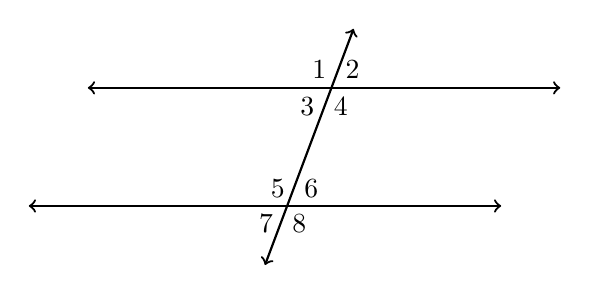
\begin{tikzpicture}[scale=.75]
  \draw [<->, thick] (1,2)--(9,2);
  \draw [<->, thick] (0,0)--(8,0);
  \draw [<->, thick] (4,-1)--(5.5,3);
  \node at (4.5,0.3) [left]{$5$};
  \node at (4.5,0.3) [right]{$6$};
  \node at (4.3,-0.3) [left]{$7$};
  \node at (4.3,-0.3) [right]{$8$};
  \node at (5.2,2) [above left]{$1$};
  \node at (5.2,2) [above right]{$2$};
  \node at (5,2) [below left]{$3$};
  \node at (5,2) [below right]{$4$};
\end{tikzpicture}
\end{center}
\begin{enumerate}
  \item State the angle corresponding with $\angle 7$. \vspace{0.5cm}
  \item What theorem would justify $m\angle 4 + m\angle 6 =180^\circ$? \rule{5cm}{0.15mm} \vspace{0.5cm}
  \item What theorem would justify $\angle 3 \cong \angle 6$? \rule{7cm}{0.15mm} \vspace{0.5cm}
  \item Given $m\angle 1 = 117^\circ$ and $m\angle 8 = (4x-3)^\circ$. Find $x$. \vspace{3.5cm}
\end{enumerate}

\end{enumerate}
\end{document}



